% I would rather have a bit of space between paragraphs
\setlength{\parskip}{0.5\baselineskip}

% I would like to include the abstract at the top
\begin{quote}
\small
\articleABSTRACT
\end{quote}


\section{Introduction}

\citet{lamichhane2003} described a Bayesian statistical method for
estimating the number and identity of essential genes in a genome from
data that indicates viable mutants. The genome of \emph{Mycobacterium
tuberculosis\/} was mutagenized with a transposon that inserted at
known sites, and a library of viable mutants was characterized. If a
mutant with insertion that disrupted a particular gene was viable,
that gene was indicated to be non-essential. Essential genes are those
for which no disruptive mutation could be viable.

The analysis method, described in further detail in
\citet{blades2002}, sought to estimate the overall proportion of
essential genes, and the probability that a gene was essential. We
assumed a uniform prior distribution on the number of essential genes,
and that genes were equally likely to be essential, and used Markov
chain Monte Carlo to derive the posterior probabilities of genes being
essential.

As part of the ReScience Ten Years Reproducibility Challenge, I sought
to reproduce the analysis in the paper, which I conducted in 2002
while an assistant professor in the Department of Biostatistics at
Johns Hopkins University. The bulk of the data and code were quickly
identified. (I keep collaborative projects in a directory
{\tt {\textasciitilde}/Projects} and save old projects in compressed form in
{\tt {\textasciitilde}/Projects/Tar}, and I immediately found
the file {\tt Gyanu.tgz}. Gyanu Lamichhane was first author on the
paper.) However, there were a number of challenges in reconstructing
the analysis steps, and the code used to conduct the computer
simulations underlying Figure~3 of \citet{lamichhane2003} appears
lost; I found only the results and the code to generate the figure.

The method was implemented in a combination of R \citep{R} and C
\citep{C} and assembled as an R package, R/negenes \citep{negenes},
which is available on both
\href{https://github.com/kbroman/negenes}{GitHub} and the
\href{https://cran.r-project.org/package=negenes}{Comprehensive R
  Archive Network (CRAN)}. The software used for the analyses in the
paper are a set of R scripts, along with one Perl script
\citep{Perl} that extracted transposon insertion sites from the \emph{M.
tuberculosis\/} genome.

\section{Challenges}

The first challenge in reproducing the analyses
in \citet{lamichhane2003} was to identify exactly what analyses needed
to be reproduced. The project directory did not contain any
documentation, and the file organization (Figure~\ref{fig:files}) was
quirky and contained a number of ancillary analyses that did not end
up in the paper. And so I had to resort to actually reading the
original article.



\begin{figure}
\definecolor{offwhite}{RGB}{255,250,240}
\lstset{language=bash,
        basicstyle=\ttfamily\scriptsize,
        frame=single,
        commentstyle=,
        backgroundcolor=\color{offwhite},
        showspaces=false,
        showstringspaces=false
        }

\begin{lstlisting}
class_problems.txt        findTA.pl*        Randomness/
Converge/                 mindGaps.pl*      Rawdata/
crucial_doubleTA.txt      Nov02/            Sept02/
Data/                     Operons/          Sims/
doubleta_hit.txt          R/                TroubleShootingSubClasses.txt
exploreSeq.pl*
\end{lstlisting}

\caption{Project directory for the work\label{fig:files}}
\end{figure}



There was some system behind the organization of the project files,
but it would have benefited from a {\tt ReadMe} file that
explained the structure. The
subdirectories {\tt Converge}, {\tt Operons}, {\tt Randomness},
and {\tt Sims} contain the ancillary analyses that did not end up in the
paper. {\tt Rawdata} contains the primary data files, {\tt Data}
contains derived data files, and {\tt R} contains analysis scripts.

But actually {\tt Rawdata}, {\tt Data}, and {\tt R} contain files
for an initial analysis of the data performed in July, 2002. The subdirectory
{\tt Sept02} contains copies of those data and scripts
for a revised analysis performed in September, 2002; many of the files
are identicial, but additional data had been added.
Similarly, {\tt Nov02} contains further copies of the data and
scripts for a further revised analysis performed in November, 2002.

The bulk of the results in the paper are those from {\tt Nov02}.
Table~2 in \citet{lamichhane2003} includes results from {\tt Sept02}
as well as {\tt Nov02}. This was the primary challenge in reproducing
the analyses: identifying which versions of the analysis
scripts were used.

There were a number of further challenges in reproducing the results.
The code to produce Figure~1b in \citet{lamichhane2003} (see
Figure~\ref{fig:fig1b}, below) was not
present in the project directory, but rather was found in a separate
directory, with files for a talk that I gave on the work.

Further, the key analyses involved Markov chain Monte Carlo (MCMC),
but I had not saved the seeds for the random number generator, and so
I am not able to reproduce the results exactly. Also, I did not save
the key intermediate results to files, and I did not indicate which
objects were produced by which scripts. Rather, I left objects in the
R environment (saved in a {\tt .RData} file and re-loaded when R was
invoked) and used them as needed without explaining where they had
come from. Nevertheless, the analysis scripts were reasonably well
named ({\tt prepareData.R}, {\tt analysis.R},
and {\tt figs4paper.R}), and so the order of the analysis could be
reconstructed without much difficulty.

\section{Code modifications}

The original analysis was performed with R version 1.5.1 (2002-06-17);
the reproduction used R version 3.6.1 (2019-07-05). The analysis
scripts could be run with only one small modification. The output of
the R function {\tt table()}, which counts the values in a
categorical variable, is now an object of class {\tt table}, and so
we needed to insert a couple of {\tt as.numeric()} calls to avoid
errors.

We also needed to make small changes regarding cutoffs controlling which results
were shown in two key tables. Because we had not saved the seed for
the random number generator, we were not able to reproduce the MCMC
results exactly, and small differences in the estimated posterior
probabilities meant that we needed to change cutoffs from 0.749 to
0.745 in order to display the same set of genes and gene families.




\section{The R/negenes package}

The key software implementing the methods of \citet{lamichhane2003}
is in the R package, R/negenes \citep{negenes}, available on the
\href{https://cran.r-project.org/package=negenes}{Comprehensive R
Archive Network (CRAN)}. The earliest version on CRAN is 0.98-3, dated
2002-08-10 and posted to CRAN on 2003-06-21. This is the version that
was used for the analyses in the paper.

There have been twelve revisions posted to CRAN. The current verison
is 1.0-12, dated 2019-08-05, and this is the version we used to
reproduce the results of the paper. The package is also available on
\href{https://github.com/kbroman/negenes}{GitHub}, though I did not
start using version control for the package until 2011-11-07.

The \href{https://github.com/kbroman/negenes/blob/master/ChangeLog}{\tt
ChangeLog} file summarizes the changes that have been made to the
package. The only substantive change was on 2012-03-09, to fix a bug
in which we were over-running an array. The problem was identified by
CRAN maintainers. Various maintence changes have been made over the
years, related to changing policies for R packages, including the
introduction of the {\tt NAMESPACE} file, which indicates
user-available functions, and registration of compiled routines. We
also changed the documentation format to use
Roxygen2 \citep{roxygen2}.


\section{Results}


\begin{table}
\caption{Reproduction of Table 2 in \citet{lamichhane2003}. The one
difference is indicated in bold.\label{tab:tab2}}

\centering
% latex table generated in R 3.6.1 by xtable 1.8-4 package
% Fri Feb 14 16:47:41 2020
\begin{tabular}{cccr@{--}lr@{--}l}
  \hline
  & \multicolumn{2}{c}{Estimate (\%)} & \multicolumn{4}{c}{95\% credible interval}\\ Rule & original & reproduction & \multicolumn{2}{c}{original} & \multicolumn{2}{c}{reproduction}\\ \hline
100\% & 34 & 34 & 27 & 39 & 27 & 39 \\ 
  90\% & 36 & 36 & 29 & 42 & 29 & 42 \\ 
  5'80\%-3'100bp & 35 & 35 & 28 & 41 & 28 & 41 \\ 
  80\% & 40 & 40 & 33 & 46 & 33 & 46 \\ 
  70\% & 42 & 42 & 35 & 49 & 35 & 49 \\ 
  60\% & 42 & 42 & 33 & 50 & 33 & \textbf{49} \\ 
   \hline
\end{tabular}

\end{table}



\begin{table}
\caption{Reproduction of Supplementary Table~6 in \citet{lamichhane2003}, which
is an expanded version of Table~3.
Genes indicated with * are the ones that were not also included in
Table 3 of \citet{lamichhane2003}.\label{tab:tab6}}

\centering
% latex table generated in R 3.6.1 by xtable 1.8-4 package
% Fri Feb 14 19:18:38 2020
\begin{tabular}{ccccc}
  \hline
  & & & \multicolumn{2}{c}{Probability (\%)}\\ MT \# & Rv \# & Gene description & original & reproduction\\ \hline
0418 & 0405 & Polyketide synthase (pks6)*  & 93 & 93 \\ 
  1218 & 1181 & Polyketide synthase  (pks4)*  & 88 & 88 \\ 
  3003 & 2933 & Phenolphthiocerol synthesis*  & 84 & 84 \\ 
  0417 & 0404 & Acyl-CoA synthase (fadD30) & 83 & 83 \\ 
  1701 & 1661 & Polyketide synthase (pks7)*  & 83 & 83 \\ 
  2062 & 2006 & Trehalose-6-phosphatase & 83 & 83 \\ 
  3285 & 3193c & Probable integral membrane protein & 83 & 83 \\ 
  2448 & 2380c & Mycobactin/Exochelin synthesis*  & 83 & 83 \\ 
  2082 & 2024c & Conserved hypothetical protein & 82 & 82 \\ 
  3974 & 3859c & Glutamate synthase (gltB) & 82 & 82 \\ 
  1587 & 1536 & Isoleucyl-tRNA synthase & 81 & 81 \\ 
  1198 & 1161 & Nitrate reductase[a]subunit (narG) & 79 & 79 \\ 
  0047 & 0041 & Leucyl-tRNA synthase (leuS) & 79 & 79 \\ 
  3002 & 2932 & Phenolphthiocerol synthesis*  & 78 & 78 \\ 
  2600 & 2524c & Fatty acid synthase (fasI) & 78 & 78 \\ 
  0070 & 0064 & Probable membrane protein & 77 & 77 \\ 
  1678 & 1640c & C-term Lysyl-tRNA synthase (lysX) & 76 & 76 \\ 
  1702 & 1662 & Polyketide synthase (pks8)*  & 76 & 76 \\ 
  2551 & 2476c & Conserved hypothetical protein & 75 & 75 \\ 
  1796 & 1753c & PPE-family protein & 75 & 75 \\ 
  0116 & 0107c & Probable Mg transport ATPase & 75 & 75 \\ 
  3045 & 2967c & Pyruvate carboxylase & 75 & 75 \\ 
   \hline
\end{tabular}

\end{table}




\begin{table}
\caption{Reproduction of Table 4 in \citet{lamichhane2003}.\label{tab:tab4}}

\centering
\small
% latex table generated in R 3.6.2 by xtable 1.8-4 package
% Sun Feb 23 09:00:36 2020
\begin{tabular}{lccc@{ (}r@{--}lc@{ (}r@{--}l}
  \hline
  & \multicolumn{2}{c}{Probability enriched (\%)} & \multicolumn{6}{c}{Est. \% essential}\\ Functional group & original & reproduction & \multicolumn{3}{c}{original} & \multicolumn{3}{c}{reproduction}\\ \hline
Aminoacyl tRNA synthases... & 97 & 97 & 54 & 32 & 76) & 54 & 32 & \textbf{\color{red} 72}) \\ 
  PE family: PGRS subfamily & 94 & \textbf{\color{red} 93} & 45 & 30 & 60) & 45 & 30 & 60) \\ 
  Purine ribonucleotide biosynthesis & 82 & 82 & 46 & 21 & 68) & 46 & 21 & 68) \\ 
  Polyketide and nonribosomal... & 80 & \textbf{\color{red} 81} & 40 & 28 & 52) & 40 & 28 & 52) \\ 
  Synthesis of fatty and mycolic acids & 78 & 78 & 42 & 23 & 62) & 42 & 23 & 62) \\ 
  Ser/Thr protein kinases and... & 75 & 75 & 43 & 21 & 64) & 43 & 21 & 64) \\ 
  Biosynthesis of molybdopterin & 75 & 75 & 42 & 20 & 65) & 42 & 20 & 65) \\ 
  Unknown proteins & 4 & 4 & 32 & 25 & 39) & 32 & 25 & 39) \\ 
  Metabolism of sulphur & 4 & \textbf{\color{red} 5} & 20 & 7 & 40) & 20 & 7 & 40) \\ 
  PPE family & 4 & 4 & 27 & 17 & 36) & 27 & 17 & \textbf{\color{red} 38}) \\ 
  Conserved membrane proteins & 0 & 0 & 10 & 0 & 24) & 10 & 0 & 24) \\ 
   \hline
\end{tabular}

\end{table}




\begin{figure}
\includegraphics[viewport=133 224 464 528, width=0.50\textwidth]{../original/Nov02/R/Figs/fig1.ps}
\hfill
\includegraphics[viewport=133 224 464 528, width=0.50\textwidth]{../reproduction/Figs/fig1.ps}

\caption{Figure 1a in \citet{lamichhane2003}. Original on left. Reproduction on right.\label{fig:fig1a}}
\end{figure}

\begin{figure}
\includegraphics[viewport=179 299 438 517, width=0.50\textwidth]{../talk/Figs/circlefig.ps}
\hfill
\includegraphics[viewport=179 299 438 517, width=0.50\textwidth]{../reproduction/Figs/circlefig.ps}

\caption{Figure 1b in \citet{lamichhane2003}. Original on left. Reproduction on right.\label{fig:fig1b}}
\end{figure}

\begin{figure}
\includegraphics[viewport=44 245 525 508, width=0.50\textwidth]{../original/Nov02/R/Figs/fig2.ps}
\hfill
\includegraphics[viewport=44 245 525 508, width=0.50\textwidth]{../reproduction/Figs/fig2.ps}

\caption{Figure 2 in \citet{lamichhane2003}. Original on left. Reproduction on right.\label{fig:fig2}}
\end{figure}


\section{Lessons}

- document your work

- use formal version control

- combine multiple mutated versions of scripts into unified versions
  that provide the comprehensive set of analysis results.

- put all relevant scripts into a common project directory

- keep track of random number generator seeds

- save intermediate results to files and then load them at the top of
  the script

- document the provenance of raw data files
